\subsection{Expérimentation}
Observons ensuite le résultat de l'apprentissage des réseaux de neurones sur les données issues de la commande aléatoire.

\newcommand{\actu}[1]{#1_{\text{actuelle}}}
\newcommand{\target}[1]{#1_{\text{target}}}
\newcommand{\xactu}{\actu{X}}
\newcommand{\yactu}{\actu{Y}}
\newcommand{\vactu}{\actu{V}}
\newcommand{\vtarget}{\target{V}}
\newcommand{\oactu}{\actu{O}}
\newcommand{\otarget}{\target{O}}
\newcommand{\mpwekawidth}{.48\linewidth}
\newcommand{\incweka}[1]{\includegraphics[scale=0.5]{#1}}
\newcommand{\wecaption}[1]{\caption{#1.\footnotesize (Généré par Weka 3.8.1)\normalsize}}
\subsubsection{Test du réseau de neurones}
Afin de vérifier si le réseau de neurones implémenté ne contient pas d'erreur, il sera d'abord utilisé pour une Sphero virtuelle.
Un modèle très simple de Sphéro a été implémenté. Ce modèle ne simule pas la vitesse et l'inertie angulaire.
Le modèle est le suivant: Soit
\begin{itemize}
 \item $(\xactu, \yactu)$ la position actuelle en cm,
 \item $\vactu$ la vitesse actuelle en cm/s
 \item $\vtarget$ la vitesse commandée d'unité inconnue,
 \item $\oactu$ l'orientation en degrés,
 \item $\otarget$ l'orientation commandée en degrés,
 \item $T$ la période de streaming.
\end{itemize}
\[ \text{acceleration} = a(\vtarget - \vactu)\]
Où $a \in \mathbb{R}^{+}$ est un paramètre.
\[ \text{Nouvelle vitesse} = \vactu + \text{acceleration} \times T \]
Posons $d$ la différence entre $\otarget$ et $\oactu$, négatif si le sens de $\oactu \rightarrow \otarget$ est horlogique.
Alors
\[ \text{Nouvelle orientation} = \oactu + d \]
Nouvelle vitesse et Nouvelle orientation sont limitées selon un paramètre.
\begin{center}
 \begin{tabular}{ll}
  Nouvelle position = & $(\xactu + (\text{Nouvelle vitesse})\cos(\text{Nouvelle orientation})$,\\
   & $\yactu + \text{Nouvelle vitesse}\sin(\text{Nouvelle orientation}))$
 \end{tabular}
\end{center}

Deux réseaux de neurones ont été testés: le \rbf implémenté et le \mlp de Weka.
La fonction d'activation des neurones cachés de Weka est la sigmoïde: 
\[ f(x) = \frac{1}{1+e^{-x}} \]
et la fonction d'activation des neurones de sortie est une fonction linéaire.\cite{mlpweka}

\begin{figure}
 \begin{minipage}[c]{\mpwekawidth}
  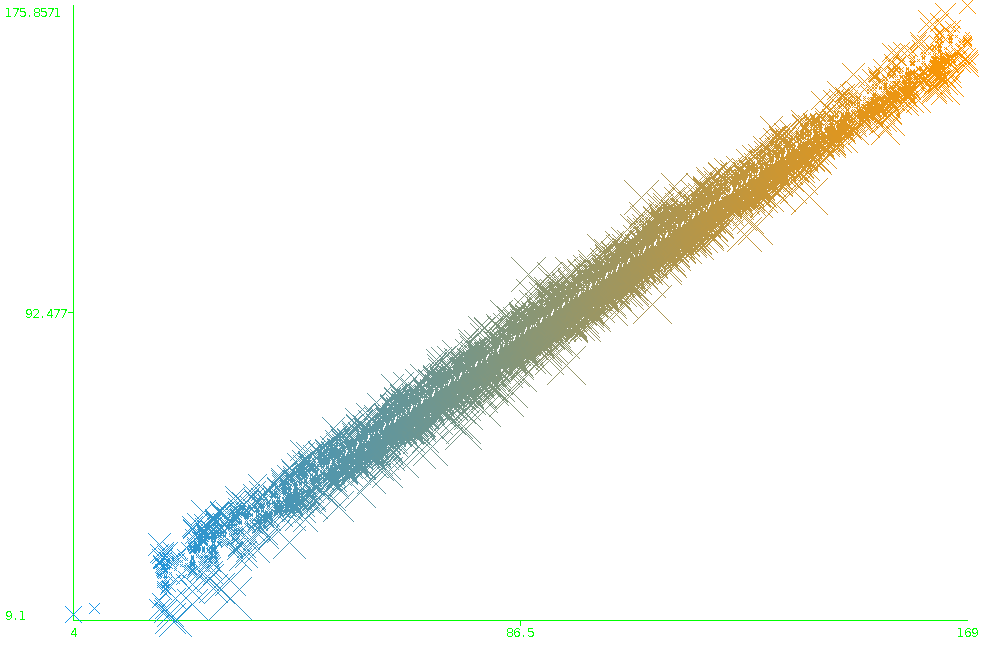
\includegraphics[width=\textwidth]{../figures/virtualResultSpeed.png}
 \end{minipage}
 \begin{minipage}[c]{\mpwekawidth}
  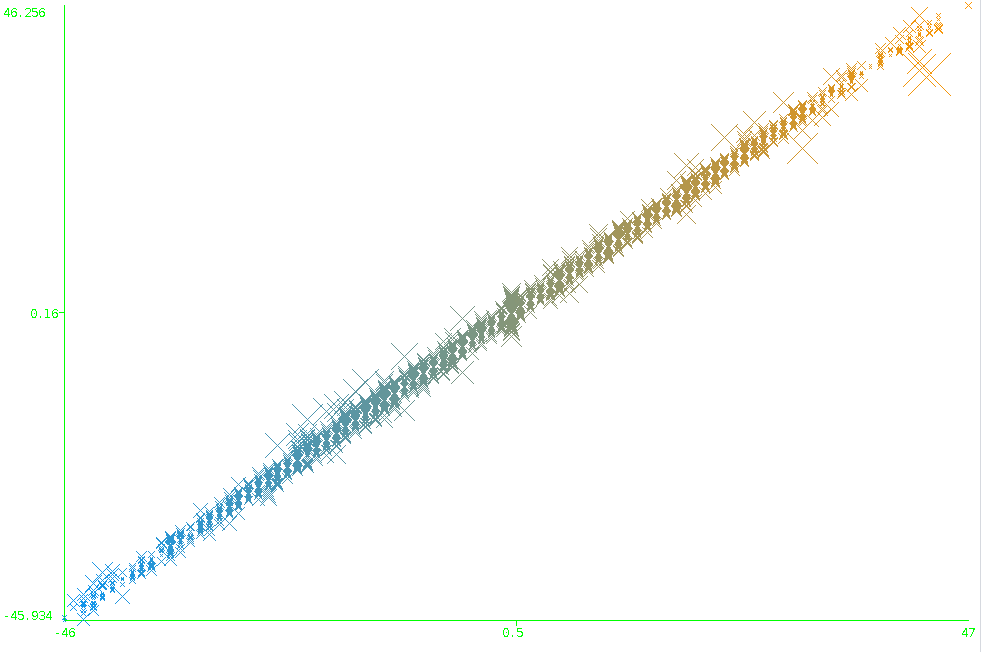
\includegraphics[width=\textwidth]{../figures/virtualHeadResult.png}
 \end{minipage}
 \wecaption{Nuages de point prédit/espéré sur la vitesse et l'orientation sur les données de la Sphero virtuelle}
 \label{we:virtualResult}
\end{figure}
Tous les deux étaient capables d'approximer ce modèle.
Pour que les résultats observés ne soient pas biaisées par le surajustement, la technique de 10fold cross-validation a été utilisée.
C'est-à-dire que la base de données est séparée en 10 ensembles de tailles égales.
Pour chaque ensemble, on construit le modèle sur les 90 autres pourcents de données et on utilise ces 10\% comme ensemble de test.
À la fin, on obtient un nuage de points (sortie espérée, sortie aproximée par le modèle) où nous pouvons, par exemple,
calculer le coefficient de corrélation pour avoir un indice sur la qualité du réseau de neurones pour ces données.
Comme sur la Figure \ref{we:virtualResult} où la corrélation est de 0,99 pour la vitesse et l'orientation.
Deux modèles différents ont été construit car il a été observé que le RBF implémenté est plus éfficace si il n'y a qu'une sortie à générer au lieu de deux.

\subsubsection{Observation des données réelles}
\begin{figure}
 \centering
 \incweka{../figures/targetxyvirtual.png}
 \wecaption{Nuage des positions et de la direction à commander pour les atteindre. Pour la Sphero virtuelle}
 \label{we:targetvirtual}
\end{figure}
\begin{figure}
 \centering
 \incweka{../figures/targetxSpeedvirtual.png}
 \wecaption{Nuage des positions et de la vitesse à commander pour les atteindre. Pour la Sphero virtuelle}
 \label{we:targetvirtualSpeed}
\end{figure}

Observons les données fournies par la commande aléatoire sur la véritable Sphero.
Dans la figure \ref{we:targetxy} et \ref{we:targetxySpeed}, chaque point représentent la position que doit atteindre la Sphero $\frac{1}{f}$ secondes plus tard.
Pour chaque point, la Sphero est en (0,0) et est dirigée vers la droite, parallèle à l'axe x.
La couleur du point représente la valeur de l'orientation à commander.
Plus le ton est orangé, plus la valeur est grande.
On pourrait s'attendre à ce que plus le point est vers le haut, plus la valeur de head est grande, comme on peut l'observer sur les données de commande aléatoire sur la Sphero virtuelle. (Figure \ref{we:targetvirtual})
On pourrait s'attendre aussi à ce que plus le point à atteindre est éloigné de la position actuelle, plus la vitesse commandée doit être élevée, comme on peut également le voir sur les données venant de la Sphero virtuelle. (Figure \ref{we:targetvirtualSpeed})

\begin{figure}
 \centering
 \incweka{../figures/targetxy.png}
 \wecaption{Nuage des positions et de la direction à commander pour les atteindre. Pour la Sphero réelle}
 \label{we:targetxy}
\end{figure}
Concernant les données de la Sphero réelle, si on prend les attributs deux à deux, on n'observe pas de pattern quant à la direction à prendre selon les données acquises.
Une de ces observation est illustrée dans la Figure \ref{we:targetxy}.
Dans cette figure, tous les points ont été légèrement déplacés aléatoirement afin de pouvoir tous les distinguer.
Nous devrions voir en plus de 3 dimensions pour observer un éventuel pattern.
Mais en tout cas, selon Wela, il y en a un.
C'est ce que nous allons voir dans \hyperref[sec:realdataex]{l'expérimentation sur les données réelles}.
Notons qu'il est possible d'obtenir des données indiquant qu'il faut tourner, par exemple, à droite pour une position qui se trouve plutôt vers la gauche.
En effet, après un virage serré, à cause de la force centrifuge exercée sur le centre de gravité, la Sphero se met à se balancer de gauche à droite par rapport à sa direction.
Juste avant la fin de ce virage, nous avons commandé à la Sphero de tourner vers la droite.
Mais à la fin de son virage, l'inertie de son centre de gravité la fait basculer vers la gauche.
Si la position est échantillonée pendant ce basculement, alors on a une position qui peut être vers la gauche par rapport à la position échantillonée juste avant alors qu'on avait commander à la Sphero de tourner vers la droite.
Ce problème est analogue aux dérapages.
Mais comme il ne s'agit pas d'un dérapage, la position réellement atteinte est effectivement échantillonée par l'odomètre.
Afin de détecter ces cas, il nous faudrait observer la vitesse ou l'accélération en plus de la position à atteindre.

\begin{figure}
 \centering
 \incweka{../figures/targetxySpeed.png}
 \wecaption{Nuage des positions et de la vitesse à commander pour les atteindre. Pour la Sphero réelle}
 \label{we:targetxySpeed}
\end{figure}
Tandis que pour la vitesse à commander, sur la Figure \ref{we:targetxySpeed} on observe effectivement une tendance à commander une vitesse plus élevée pour atteindre des positions plus éloignées.
Plus la couleur du point est orangée, plus la vitesse est élevée.

\subsubsection{Expérimentation sur données réelles}\label{sec:realdataex}
Puisque cette expérience s'est déroulée en même temps que la phase de conception et de test du générateur de commande aléatoire,
il a fallut préparer un espace accessible sur une assez longue période.
La vitesse a été bridée et aucune caméra n'a été utilisée.
Dans ces conditions, une fréquence de 40Hz était trop élevée pour capturer les différences de positions car l'odométrie est capturée en nombre entier en cm.
Une fréquence de 5Hz était assez basse pour observer les différences de position mais assez élevée pour effectuer des mouvements fluides.
Pour toutes les obsevations effectuées, le RBF implémenté retournait toujours la moyenne des outputs.

\ssstitle{Avec données relatives à la position et l'orientation}
\begin{minipage}[c]{\mpwekawidth}
 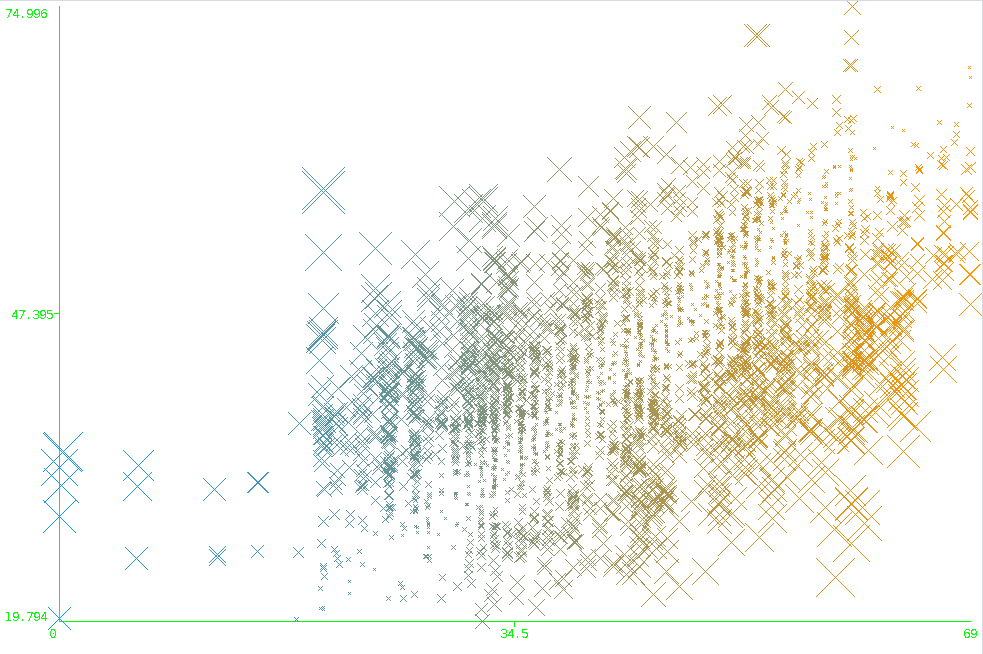
\includegraphics[width=\textwidth]{../figures/speed121314N1500H20.png}
 \begin{center}
  \textbf{Vitesse}
 \end{center}
\end{minipage}
\begin{minipage}[c]{\mpwekawidth}
 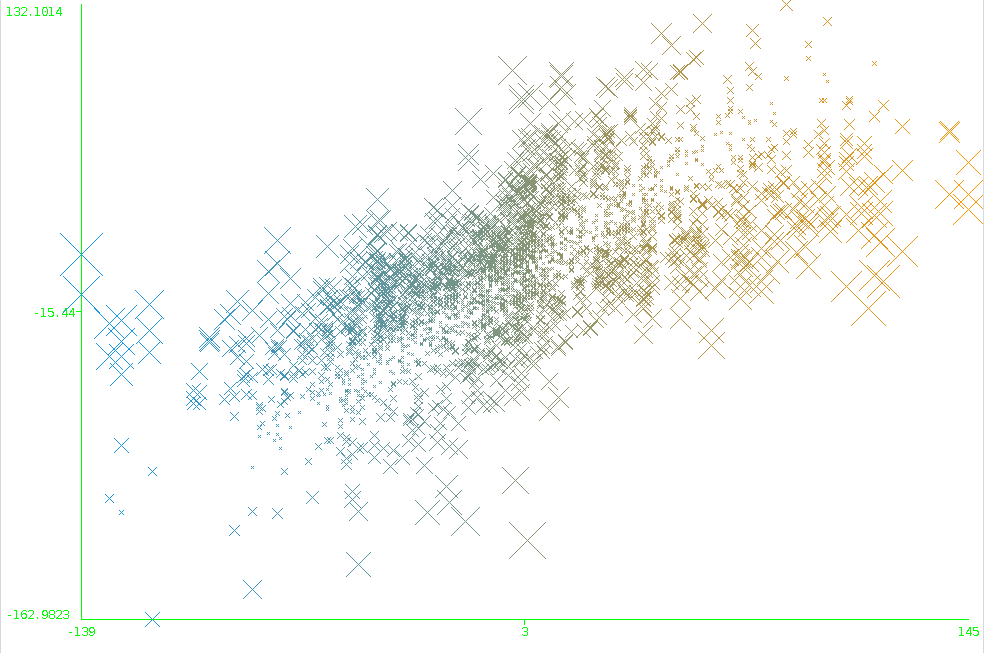
\includegraphics[width=\textwidth]{../figures/121314N1500H20.png}
 \begin{center}
  \textbf{Orientation}
 \end{center}
\end{minipage}
\\

Ici, les données d'entrées sont relatives à la position de la Sphero et à son orientation.
Les données sont normalisées avant des les utiliser dans le réseau de neurones.
Si les valeurs de sortie ne sont pas normalisées, alors si elles ont un domaine différent, elles n'auront pas le même poids lors du calcul d'erreur.
Si les valeurs d'entrée ne sont pas normalisées, alors nous devons paramètrer nous-mêmes l'initialisation de certains neurones.
Comme les neurones du RBF, si ils sont initialisés avec un écart-type de 1 et une moyenne de 0 mais que les valeurs d'entrées peuvent atteindre plusieurs centaines,
alors malgré la précision en 64bits du calcul de la fonction d'activation, elles retourneront souvent 0.
Idem pour la fonction sigmoïde, elle retourna souvent 0 ou 1.

En construisant le modèle en règlant les paramètres, un optimum local a été atteint sur Weka. Il s'agit d'une seule couche de 20 neurones cachés avec un learning rate (i.e. pas de gradient) de 0,3 et un nombre d'époques de 1500.
(C'est-à-dire que les données d'entrainement sont présentés 1500 fois aux réseaux de neurones).
Le coefficient de corrélation du modèle construit par Weka est de 0.5404 pour la vitesse et de 0,69 pour l'orientation.

\ssstitle{Sans normalisation des données}
\begin{minipage}[c]{\mpwekawidth}
 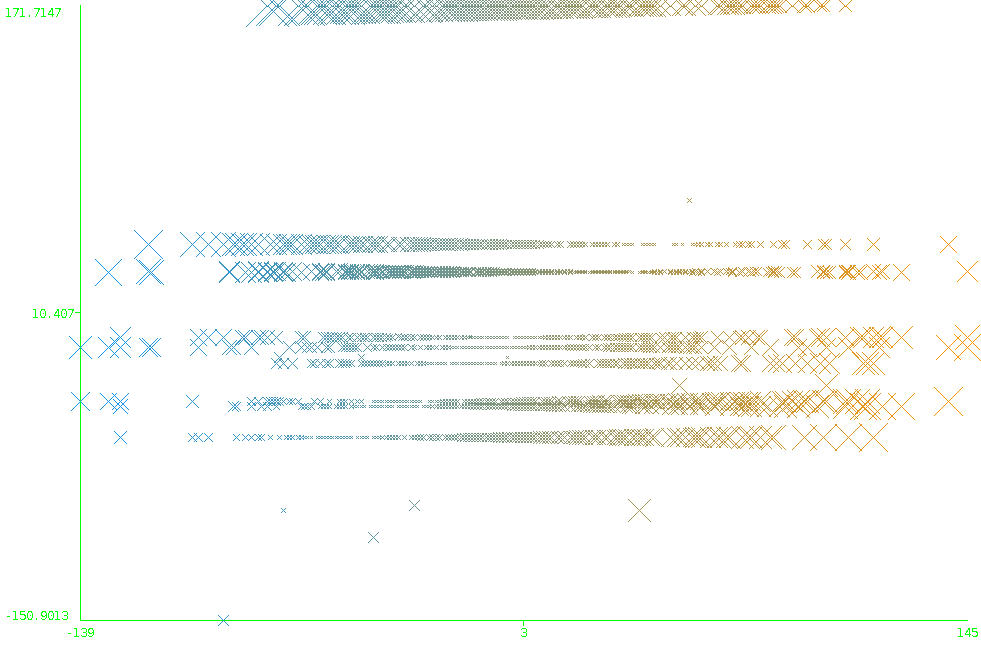
\includegraphics[width=\textwidth]{../figures/121314SpeedOutputNotNormalized.png}
 \begin{center}
  \textbf{Vitesse}
 \end{center}
\end{minipage}
\begin{minipage}[c]{\mpwekawidth}
 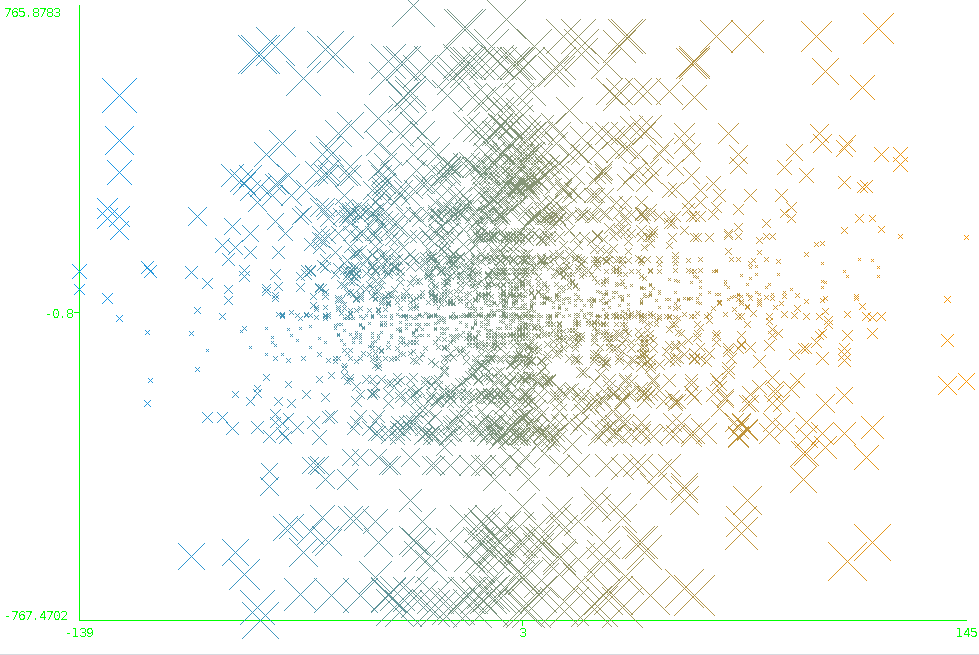
\includegraphics[width=\textwidth]{../figures/HeadNotNormalized.png}
 \begin{center}
  \textbf{Orientation}
 \end{center}
\end{minipage}
\\

Si nous n'avions pas normalisé les données, le coefficient de corrélation du modèle construit par Weka est de 0,0119 pour la vitesse et 0,0264 pour l'orientation.
Nous pouvons d'ailleur ci-dessus observer un comportement étrange sur les prédictions données par le modèle.
La configuration du réseau de neurones est la même que la précédente.

\ssstitle{Ajout de la vitesse commandée en attribut}
\incweka{../figures/121314SpeedN1500H20.png}
\\

Revenons aux données normalisées et ajoutons la vitesse commandée en attribut.
Toujours avec la même configuration du réseau de neurones.
Puisque nous pouvons utiliser un réseau différent pas sortie, il est possible de d'abord prédire la vitesse à commander et d'ensuite ajouter cette donnée pour la prédiction de l'orientation à prendre si celle-ci améliore la précision.
Dans ce cas, le coefficient de corrélation atteint 0,72 pour l'orientation.
Un test est nécessaire afin de confirmer si cette augmentation de 0,03 est significatif.
Par ailleur, si on ajoute l'orientation commandée comme attribut pour le modèle prédisant la vitesse à commander, la corrélation est de 0,4991.

\ssstitle{En considérant la symétrie orthogonale}
Dans la section \ref{sec:choixdesign} nous avons évoquer une possibilité d'une symétrie orthogonale d'axe x sur l'orientation et la vitesse à prendre.
C'est d'ailleur ce qui est observé sur les données de la Sphero virtuelle, Figure \ref{we:targetvirtual} et \ref{we:targetvirtualSpeed}.
Nous allons le vérifier pour les données réelles.
Pour chaque instance, si l'ordonnée de la position à atteindre est négatif, on multiplie par -1 toutes les ordonnées des entrées.
C'est-à-dire que si targety est <0, alors targety = -targety, currentSpeedy = -currentSpeedy et currentAccely = -currentAccely.
Toujours avec la même configuration de réseau, le coefficient de corrélation devient 0,5123 pour la vitesse et 0,6339 pour l'orientation.

\ssstitle{Résultats étranges avec le one nearest neighbor}
\begin{minipage}[c]{\mpwekawidth}
 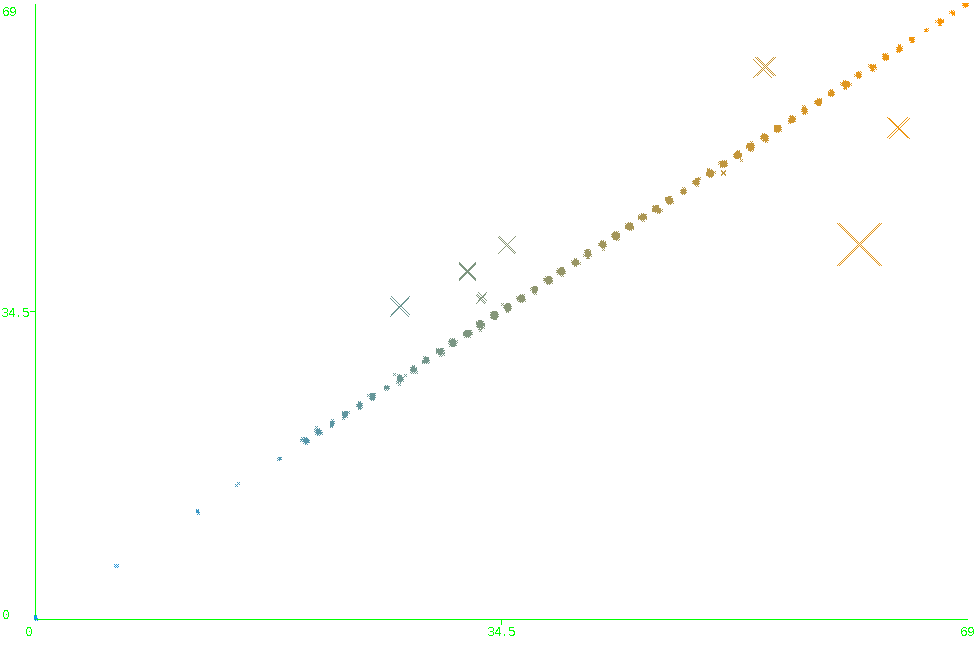
\includegraphics[width=\textwidth]{../figures/1BkSpeed.png}
 \begin{center}
  \textbf{Vitesse}
 \end{center}
\end{minipage}
\begin{minipage}[c]{\mpwekawidth}
 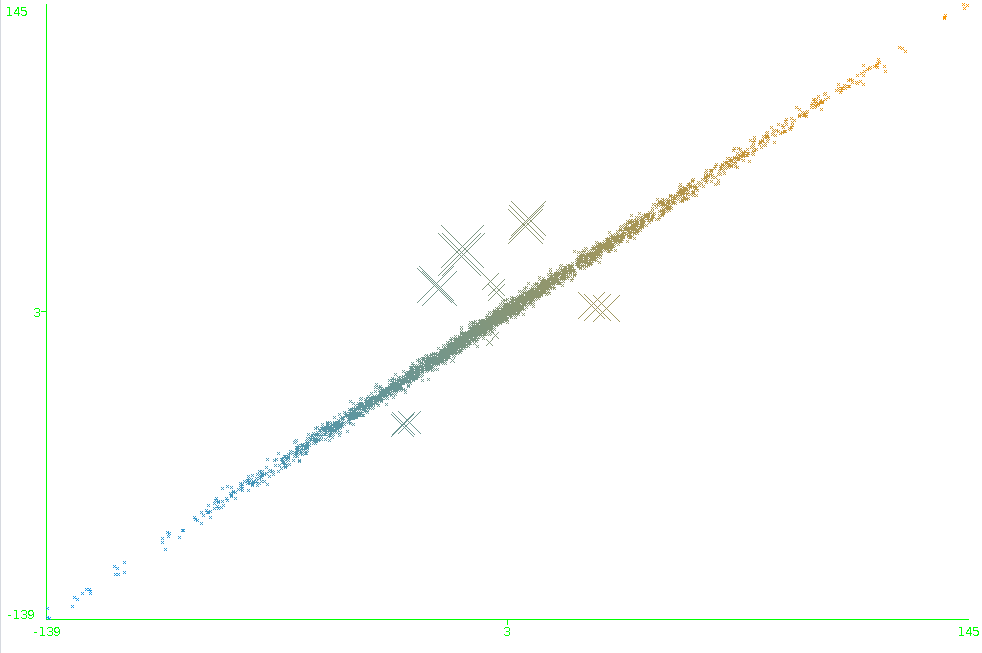
\includegraphics[width=\textwidth]{../figures/IB1.png}
 \begin{center}
  \textbf{Orientation}
 \end{center}
\end{minipage}
\\

Des résultats étranges ont été observés lorsque un modèle de régression est construit par le \emph{one nearest neighbor} sur ces données via Weka.
Pour prédire une valeur à partir des entrées, le modèle effectue un calcul de distance entre ces entrées et toutes les entrées des instances de l'ensemble d'apprentissage.
Ensuite il retient l'instance la plus proche et retourne sa sortie.
Ce modèle utilise des données normalisées.
La corrélation atteint 0,9977 pour la vitesse et 0,9985 pour l'orientation !
Rappelons que par le principe du 10cross validation, aucune instance de test n'est reprise dans les instances d'entrainement.

Le one nearest neighbor a été implémenté dans le commander et testé sur les mêmes données utilisées dans Weka.
Pour la validation, le $N$cross validation a été appliqué où $N$ est le nombre d'instance.
Les modèles générés devraient donc être théoriquement plus performant que ceux construits durant un 10cross validation.
Mais on observe une corrélation de ? pour la vitesse et ? pour l'orientation.
Au vu de ces résultats, nous pouvons avoir des doutes quant aux résultats des modèles de réseaux de neurones produits pas Weka.

\subsubsection{Déploiement}
Nous avons donc trouvé un réseau de neurones convergeant vers une solution de corrélation de plus de 0,50 entre la vitesse à commander prédite et celle qui est attendue et de presque 0,70 pour l'orientation à commander.
Au lieu d'implémenter le même réseau pour le commander, utiliser une API de réseau de neurones nous permetra de modifier plus rapidement la configuration du réseau et de tester de nouveaux types de réseau.
L'API choisie est Caffe elle permet de mofidier aisément l'architecture via un fichier texte au format prototxt.\cite{caffe}
Les paramètres du modèle comme le nombre d'époques ou le pas de gradient peuvent aussi être modifiée via un tel fichier.
De plus, étant en c++, le réseau peut rapidement être intégré dans l'impémentation actuelle du commander.
L'enregistrement et le chargement d'un modèle est entièrement pris en charge par Caffe et ne dépend pas de l'architecture.
Et enfin, l'implémentation de Caffe est multithreadé.

Avec ce nouveau réseau de neurones, les performances du commander sur les données de la Sphero virtuelle sont bonnes. %TODO montrer
Malheureusement, avec les données de la Sphero réelle, ce modèle converge vers la moyenne de toutes les sorties à prédire. %TODO et sur la vitesse ?